% Provenance (never printed): see sources/outline_sources.md (Year 3: refraction and
% reflection seismic methods; CMP acquisition, NMO, stacking, Dix; migration in
% principle; seismic stratigraphy). Brief: sources/book5/BRIEFS.md, ch. 2. Curves from
% figdata/bachelor-3/seismic_model.py, refraction_dip.py, synthetic_seismogram.py,
% cmp_nmo.py (the Varden column, region.py); exercise and problem values in the
% Book 5 scratch calculator calc/ch02.py.
\chapter{Sismología de exploración}\label{ch:b3:exploration-seismology}

Un buque de prospección avanza lentamente en línea recta por el mar, remolcando un conjunto de cañones de aire
a pocos metros bajo la superficie y, detrás de él, cables de varios
kilómetros de longitud provistos de hidrófonos. En una prospección descrita ante el
regulador, el conjunto contenía \num{5240} pulgadas cúbicas de aire comprimido, disparado cada
\qty{8}{s} desde \qty{12}{m} bajo la superficie, y los cables remolcados de acimut estrecho
detrás de tales buques registran offsets de entre 8 y \qty{10}{km}.
% ledger: noaa5:wg-survey
Cada disparo envía un pulso de sonido al fondo marino, y cada interfaz rocosa
situada debajo devuelve un eco débil. Semanas de procesado después, un geólogo recorre
una sección en la que aparecen canales fluviales enterrados, bloques de falla basculados y
el relleno en \omterm{def:b3:exploration-seismology:terminations}{onlap} de una antigua cuenca aparecen como si el terreno se hubiera abierto en corte.
La sismología a escala terrestre del capítulo anterior utilizaba las ondas de
terremotos; la sismología de exploración genera las propias, con fuentes cuyo instante y
lugar se conocen con exactitud y las registra en miles de canales. Este
capítulo sigue los ecos desde el disparo hasta la sección: prospecciones de refracción,
la reflexión de una ondícula en una columna estratificada, el método del \omterm{def:b3:exploration-seismology:cmp}{punto medio común}
que convierte ecos repetidos en velocidades y en una imagen nítida, la \omterm{def:b3:exploration-seismology:migration}{migración sísmica}, que
devuelve los reflectores a su posición correcta, y la lectura de la sección como
\omterm{def:b3:exploration-seismology:seismic-stratigraphy}{estratigrafía sísmica}.

\begin{recall}
En la frontera entre dos medios de impedancia acústica $Z_1 = \rho_1v_1$ y
$Z_2 = \rho_2v_2$, una onda plana con incidencia normal se refleja con el
coeficiente de amplitud $R = (Z_2 - Z_1)/(Z_2 + Z_1)$ (en el volumen de segundo año de
los libros de física, sobre ondas en interfaces). La onda de cabeza, el tiempo de intercepción y la
distancia de cruce de un perfil de refracción sobre capas planas se estudiaron en el
volumen de primer año, en su capítulo sobre la Tierra estratificada; los registros de sondeo del
libro 2 (año 11). La convolución $(f*g)(t) = \int f(\tau)g(t - \tau)\,\mathrm d\tau$
y la transformada de Fourier son de los libros de matemáticas. El \omterm{def:b3:seismology-imaging:ray-parameter}{parámetro del rayo} y el
\omterm{def:b3:seismology-imaging:inverse}{problema inverso} lineal son los del \cref{ch:b3:seismology-imaging}.
\end{recall}

\section{Prospecciones de refracción}

\begin{definition}[Prospecciones sísmicas de refracción y de reflexión]\label{def:b3:exploration-seismology:surveys}
Una \emph{prospección sísmica de refracción}\index{prospección sísmica de refracción} registra, a lo largo
de una línea de receptores, las primeras llegadas de una fuente controlada, y utiliza las
ondas de cabeza que viajan por la parte superior de las capas más rápidas para determinar sus velocidades y
profundidades. Una \emph{prospección sísmica de reflexión}\index{prospección sísmica de reflexión}
registra el tren de ondas completo, a offsets en su mayoría menores que las profundidades de
interés, y utiliza las ondas reflejadas con incidencia casi normal por las
interfaces para obtener una imagen de la estratificación.
\end{definition}

Sobre capas planas, una onda de cabeza llega en $t = x/v_2 + t_i$, una recta
cuya pendiente da la velocidad $v_2$ del refractor y cuya ordenada en el origen $t_i$
da su profundidad. Un refractor con buzamiento inclina la recta: la onda de cabeza disparada
en sentido de buzamiento llega cada vez más tarde, a medida que el refractor se hunde, y parece lenta;
disparada en contra del buzamiento parece rápida. Disparando en ambos sentidos a lo largo de la misma línea, un perfil invertido
separa la velocidad del buzamiento.

\begin{theorem}[Refracción en una interfaz con buzamiento]\label{thm:b3:exploration-seismology:dipping}
Una capa de velocidad $v_1$ yace sobre un refractor plano de velocidad $v_2 > v_1$ que buza
con un ángulo $\theta$ a lo largo del perfil; $i_c = \arcsin(v_1/v_2)$, y $h$ es la
profundidad perpendicular del refractor bajo el disparo. Más allá de la
distancia crítica, la onda de cabeza llega en
\begin{align*}
  t &= \frac{x\sin(i_c + \theta)}{v_1} + \frac{2h\cos i_c}{v_1}
  &&\text{disparo en sentido de buzamiento},\\
  t &= \frac{x\sin(i_c - \theta)}{v_1} + \frac{2h\cos i_c}{v_1}
  &&\text{disparo en contra del buzamiento}.
\end{align*}
Las velocidades aparentes $v_d = v_1/\sin(i_c + \theta)$ y
$v_u = v_1/\sin(i_c - \theta)$ de un perfil invertido dan
\[
  i_c = \tfrac12\left[\arcsin\frac{v_1}{v_d} + \arcsin\frac{v_1}{v_u}\right],\qquad
  \theta = \tfrac12\left[\arcsin\frac{v_1}{v_d} - \arcsin\frac{v_1}{v_u}\right],
  \qquad v_2 = \frac{v_1}{\sin i_c} .
\]
\end{theorem}

\begin{proof}
Se gira el sistema de referencia para que el refractor quede horizontal; la superficie buza entonces
$\theta$, y disparando en sentido de buzamiento, la profundidad perpendicular bajo un receptor a
offset $x$ es $h + x\sin\theta$, su proyección sobre el refractor
$x\cos\theta$. La trayectoria de la onda de cabeza desciende con el ángulo crítico $i_c$ hasta la
normal, recorre el refractor a $v_2$ y asciende con $i_c$. Su tiempo es
\[
  t = \frac{h}{v_1\cos i_c} + \frac{x\cos\theta - h\tan i_c - (h + x\sin\theta)\tan i_c}{v_2}
  + \frac{h + x\sin\theta}{v_1\cos i_c}.
\]
Con $1/v_2 = \sin i_c/v_1$ y $1/\cos i_c - \sin i_c\tan i_c = \cos i_c$,
los términos en $h$ dan $2h\cos i_c/v_1$ y los de $x$ dan
  $x(\sin i_c\cos\theta + \cos i_c\sin\theta)/v_1 = x\sin(i_c + \theta)/v_1$.
En sentido contrario al buzamiento, $\theta$ cambia de signo. Las últimas fórmulas invierten las dos
velocidades aparentes.
\end{proof}

Las dos ramas de un perfil invertido deben dar el mismo tiempo entre los dos
puntos de disparo, desde cualquiera de los extremos: el \emph{tiempo recíproco}, una comprobación de la
lectura de las llegadas. Dos situaciones invalidan el método. Una capa más lenta que la que tiene encima
(una inversión de velocidad) no genera ninguna onda de cabeza y resulta invisible: sus rocas se
cuentan en la capa superior, y todas las profundidades situadas debajo quedan sobreestimadas. Una capa
más rápida que la superior pero demasiado delgada puede no dar nunca una primera llegada, porque
la onda de cabeza de la capa más profunda y rápida la alcanza: una capa oculta. Una
prospección de reflexión detecta las dos.

\begin{omfigure}
\begin{tikzpicture}
\begin{axis}[omrecord, width=0.82\linewidth, height=0.46\linewidth,
  xmin=0, xmax=1200, ymin=0, ymax=660,
  xlabel={posición a lo largo del tendido, desde el disparo O (\unit{m})},
  ylabel={tiempo (\unit{ms})}, legend pos=north west, legend cell align=left,
  legend style={font=\scriptsize}]
\addplot[gray, thick, densely dashed] table[x=x, y=tdir] {figdata/out/bachelor-3-refraction_dip-west.dat};
\addlegendentry{ondas directas ($v_1$)}
\addplot[blue!70!black, thick] table[x=x, y=thead] {figdata/out/bachelor-3-refraction_dip-west.dat};
\addlegendentry{onda de cabeza desde O, disparo en contra del buzamiento}
\addplot[red!70!black, thick] table[x expr=1200-\thisrow{x}, y=thead] {figdata/out/bachelor-3-refraction_dip-east.dat};
\addlegendentry{onda de cabeza desde E, disparo en sentido de buzamiento}
\addplot[gray, thick, densely dashed, forget plot] table[x expr=1200-\thisrow{x}, y=tdir] {figdata/out/bachelor-3-refraction_dip-east.dat};
\addplot[only marks, mark=*, mark size=1.5pt] coordinates {(1200,486.13) (0,486.13)};
\node[font=\scriptsize, anchor=south east] at (axis cs:1190,530) {tiempo recíproco};
\end{axis}
\end{tikzpicture}

\par\smallskip{\small Un perfil de refracción invertido en el flanco occidental del
anticlinal de Varden (calculado; problema, parte I). El refractor, el techo de
la caliza, asciende de O a E con un buzamiento de \ang{10.8} bajo un tendido de
\qty{1200}{m}; la creta y la lutita situadas encima se agrupan en una única capa
de \qty{2.40}{km.s^{-1}}. La onda de cabeza lanzada desde el O, en sentido
ascendente del buzamiento, resulta rápida (\qty{6.57}{km.s^{-1}}); la lanzada
desde el E, en sentido descendente, es lenta (\qty{3.52}{km.s^{-1}}), y ambas tardan
\qty{486.1}{ms} en recorrer todo el tendido. Las ondas de cabeza sobrepasan a las ondas directas solo cerca del extremo lejano: el refractor está profundo para un tendido tan corto.}
\label{fig:b3:exploration-seismology:refraction}
\end{omfigure}

\section{Reflexión a incidencia normal}

\begin{definition}[Ondícula sísmica, ondícula de Ricker]\label{def:b3:exploration-seismology:wavelet}
Una \emph{ondícula sísmica}\index{ondícula sísmica} es el pulso breve, de unas
decenas de milisegundos de duración, que la fuente y el sistema de registro
envían a través del terreno; cada reflector devuelve una copia escalada de él. La \emph{ondícula
de Ricker}\index{ondícula de Ricker} de frecuencia de pico $f$ es el pulso de fase cero
\[
  w(t) = \left(1 - 2\pi^2f^2t^2\right)e^{-\pi^2f^2t^2},
\]
la segunda derivada de una gaussiana, salvo signo y escala: un pico central y
dos lóbulos laterales, con media nula y un espectro de amplitud que alcanza su máximo en $f$.
\end{definition}

\begin{definition}[Serie de reflectividad]\label{def:b3:exploration-seismology:synthetic}
La \emph{serie de reflectividad}\index{serie de reflectividad} de una columna
estratificada es la sucesión de los coeficientes de reflexión a incidencia normal $r_k$ de sus interfases,
colocados en sus tiempos verticales de ida y vuelta $\tau_k = \sum_{i \le k} 2h_i/v_i$:
$r(t) = \sum_k r_k\,\delta(t - \tau_k)$.
\end{definition}

\begin{proposition}[El modelo convolucional]\label{prop:b3:exploration-seismology:synthetic}
Si solo se conservan las reflexiones primarias (sin múltiples), a incidencia
normal, sin pérdida por transmisión, atenuación ni divergencia, y si la ondícula
$w$ no cambia con la profundidad, el registro es la convolución de la ondícula
con la \omterm{def:b3:exploration-seismology:synthetic}{serie de reflectividad}:
\[
  s(t) = \sum_k r_k\,w(t - \tau_k) = (w*r)(t) .
\]
La traza calculada de este modo a partir de un registro de sondeo de velocidad y
densidad es el \emph{sismograma sintético}\index{sismograma sintético} del registro.
\end{proposition}

\begin{proof}
Cada interfase devuelve una copia de la ondícula incidente escalada por su
coeficiente y retardada por su tiempo de ida y vuelta; el registro es lineal, de modo que las copias se suman.
La suma es la convolución de $w$ con el tren de impulsos de Dirac ponderados
$r(t)$, puesto que $w*\delta(\cdot - \tau_k) = w(\cdot - \tau_k)$.
\end{proof}

El \omterm{prop:b3:exploration-seismology:synthetic}{sismograma sintético} es la forma en que un sondeo se vincula con una sección
sísmica: una reflexión de la sección se asocia con la interfase del registro que
la produce. La columna de Varden bajo el eje del sinclinal del problema (el modelo
sísmico de este capítulo, con velocidades y densidades elegidas dentro de los
intervalos publicados para cada roca)
% ledger: mavko:velocities
da la figura siguiente. La interfase creta--lutita refleja solo el
\qty{2.8}{\percent} de la amplitud, porque la creta y la lutita tienen casi la
misma impedancia; el techo de la caliza refleja el \qty{38}{\percent}, la base de
la caliza devuelve un pulso invertido, y el basamento, uno intenso y
positivo.

\begin{omfigure}
\begin{tikzpicture}
\begin{groupplot}[group style={group size=3 by 1, horizontal sep=0.45cm, y descriptions at=edge left},
  width=0.36\linewidth, height=0.6\linewidth, y dir=reverse, ymin=0.4, ymax=0.85,
  tick label style={font=\scriptsize}, label style={font=\small}, title style={font=\small}]
\nextgroupplot[title={impedancia}, xlabel={\scriptsize $10^6$\,\unit{kg.m^{-2}.s^{-1}}},
  ylabel={tiempo de ida y vuelta (\unit{s})}, xmin=4, xmax=14]
\addplot[black, thick] table[x=imp, y=t] {figdata/out/bachelor-3-synthetic_seismogram-log.dat};
\node[font=\tiny, anchor=west] at (axis cs:5.1,0.45) {creta};
\node[font=\tiny, anchor=west] at (axis cs:5.4,0.535) {lutita};
\node[font=\tiny, anchor=east] at (axis cs:11.6,0.62) {caliza};
\node[font=\tiny, anchor=west] at (axis cs:7.0,0.70) {arenisca};
\node[font=\tiny, anchor=east] at (axis cs:13.1,0.79) {esquisto};
\nextgroupplot[title={reflectividad}, xmin=-0.45, xmax=0.45, xtick={-0.4,0,0.4}]
\addplot[xcomb, red!70!black, thick, mark=*, mark size=1.2pt] table[x=r, y=t] {figdata/out/bachelor-3-synthetic_seismogram-refl.dat};
\draw[gray] (axis cs:0,0.4) -- (axis cs:0,0.85);
\nextgroupplot[title={traza sintética}, xmin=-0.45, xmax=0.45, xtick={-0.4,0,0.4}]
\addplot[blue!70!black, thick] table[x=s, y=t] {figdata/out/bachelor-3-synthetic_seismogram-trace.dat};
\draw[gray] (axis cs:0,0.4) -- (axis cs:0,0.85);
\end{groupplot}
\end{tikzpicture}

\par\smallskip{\small Un \omterm{prop:b3:exploration-seismology:synthetic}{sismograma sintético} de la columna de Varden bajo el
eje del sinclinal (calculado). Izquierda: la impedancia de cada capa frente al
tiempo de ida y vuelta. Centro: la \omterm{def:b3:exploration-seismology:synthetic}{serie de reflectividad}, un pico por interfase
(los tallos apuntan a la derecha si la impedancia aumenta). Derecha: su convolución con una
\omterm{def:b3:exploration-seismology:wavelet}{ondícula de Ricker} de \qty{30}{Hz}. Cada reflexión es una copia de la ondícula; la
reflexión creta--lutita, débil, a \qty{0.488}{s}, apenas es visible.}
\label{fig:b3:exploration-seismology:synthetic}
\end{omfigure}

¿Hasta qué espesor pueden seguir resolviendo las reflexiones una capa? Su techo y su base
devuelven cada uno una ondícula; cuando se solapan, interfieren.

\begin{definition}[Espesor de sintonía]\label{def:b3:exploration-seismology:resolution}
El \emph{espesor de sintonía}\index{espesor de sintonía} de un estrato es el
espesor para el que las reflexiones de su techo y de su base, de signo opuesto,
interfieren más constructivamente, de modo que la amplitud compuesta es máxima. Los estratos más delgados
no se resuelven: su techo y su base ya no pueden distinguirse por separado, y la
amplitud disminuye en proporción al espesor.
\end{definition}

\begin{proposition}[Regla del cuarto de longitud de onda]\label{prop:b3:exploration-seismology:tuning}
Para una ondícula de periodo dominante $T$ en un estrato de velocidad $v$, con
coeficientes de reflexión $+R$ en su techo y $-R$ en su base, la reflexión
compuesta es máxima cuando el espesor del estrato es $b = \lambda/4$, donde
$\lambda = vT$; para $b \ll \lambda/4$ su amplitud es proporcional a $b$.
\end{proposition}

\begin{proof}
Se representa la ondícula por su armónico dominante $\cos(2\pi t/T)$. Las dos
reflexiones son $R\cos(2\pi t/T) - R\cos(2\pi(t - \Delta t)/T)$ con
$\Delta t = 2b/v$, cuya amplitud es $2R|\sin(\pi\Delta t/T)|$: máxima para
$\Delta t = T/2$, es decir, $b = vT/4$; para $\Delta t$ pequeño es aproximadamente
$2\pi R\Delta t/T = 4\pi Rb/\lambda$.
\end{proof}

Una \omterm{def:b3:exploration-seismology:wavelet}{ondícula de Ricker} no es un armónico, y su \omterm{def:b3:exploration-seismology:resolution}{espesor de sintonía}, leído en el
modelo de cuña de la figura siguiente, es algo menor que un cuarto de la longitud
de onda a la frecuencia de pico: \qty{19.5}{m} a \qty{30}{Hz} en roca de
\qty{3000}{m.s^{-1}}, para $\lambda/4 = \qty{25}{m}$. Los datos sísmicos rara vez contienen
mucha energía por encima de unas pocas decenas de hercios procedente de profundidades de kilómetros, porque las
rocas absorben las altas frecuencias; los estratos de menos de unos \qty{20}{m} de espesor se
registran como una única reflexión.

\begin{omfigure}
\begin{tikzpicture}
\begin{axis}[omrecord, width=0.74\linewidth, height=0.42\linewidth,
  xmin=0, xmax=80, ymin=0, ymax=1.8,
  xlabel={espesor del estrato $b$ (\unit{m})}, ylabel={amplitud de pico / $R$}]
\addplot[blue!70!black, thick] table[x=b, y expr=2*\thisrow{amp}] {figdata/out/bachelor-3-synthetic_seismogram-wedge.dat};
\draw[red!70!black, densely dashed] (axis cs:19.5,0) -- (axis cs:19.5,1.6);
\node[font=\scriptsize, anchor=south, red!70!black] at (axis cs:19.5,1.6) {sintonía, \qty{19.5}{m}};
\draw[gray, densely dotted] (axis cs:25,0) -- (axis cs:25,1.6);
\node[font=\scriptsize, anchor=west, gray!40!black] at (axis cs:25.5,0.3) {$\lambda/4 = \qty{25}{m}$};
\draw[gray] (axis cs:0,1) -- (axis cs:80,1);
\node[font=\scriptsize, anchor=south east] at (axis cs:79,1) {dos ondículas separadas};
\end{axis}
\end{tikzpicture}

\par\smallskip{\small El modelo de cuña (calculado): un estrato de
\qty{3000}{m.s^{-1}} con coeficientes de reflexión $+R$ en su techo y $-R$ en
su base, registrado con una \omterm{def:b3:exploration-seismology:wavelet}{ondícula de Ricker} de \qty{30}{Hz}. La amplitud de pico de la
reflexión compuesta, relativa a una reflexión única de coeficiente $R$, crece linealmente desde cero para estratos muy delgados,
alcanza su máximo en el \omterm{def:b3:exploration-seismology:resolution}{espesor de sintonía} y se estabiliza en el nivel de dos ondículas separadas
para estratos gruesos.}
\label{fig:b3:exploration-seismology:wedge}
\end{omfigure}

Lateralmente, la resolución viene fijada por la anchura del reflector que devuelve
la energía en fase.

\begin{definition}[Zona de Fresnel]\label{def:b3:exploration-seismology:fresnel}
La \emph{zona de Fresnel}\index{zona de Fresnel} (primera) de un reflector, para
una fuente y un receptor coincidentes a una altura $z$ sobre él, es el disco del reflector
alrededor del punto de incidencia normal desde el cual el camino de ida y vuelta es más largo que el normal en
menos de media longitud de onda: sus reflexiones llegan en fase y
construyen juntas la reflexión registrada.
\end{definition}

\begin{proposition}[Radio de la zona de Fresnel]\label{prop:b3:exploration-seismology:fresnel}
La primera \omterm{def:b3:exploration-seismology:fresnel}{zona de Fresnel} tiene el radio
$r_F = \sqrt{\lambda z/2 + \lambda^2/16} \approx \sqrt{\lambda z/2}$ para
$\lambda \ll z$.
\end{proposition}

\begin{proof}
Un punto del reflector a la distancia $r$ del punto de incidencia normal se
encuentra a la distancia $\sqrt{z^2 + r^2}$ de la fuente. El exceso de camino de ida y vuelta es
$2(\sqrt{z^2 + r^2} - z)$; igualándolo a $\lambda/2$ se obtiene
$\sqrt{z^2 + r^2} = z + \lambda/4$, de donde $r^2 = \lambda z/2 + \lambda^2/16$.
\end{proof}

A \qty{1}{km} de profundidad, con $\lambda = \qty{100}{m}$, la \omterm{def:b3:exploration-seismology:fresnel}{zona de Fresnel} tiene
un radio de \qty{225}{m}: los rasgos más estrechos que eso quedan emborronados,
a menos que la migración (más abajo) concentre la zona.

\begin{omfigure}
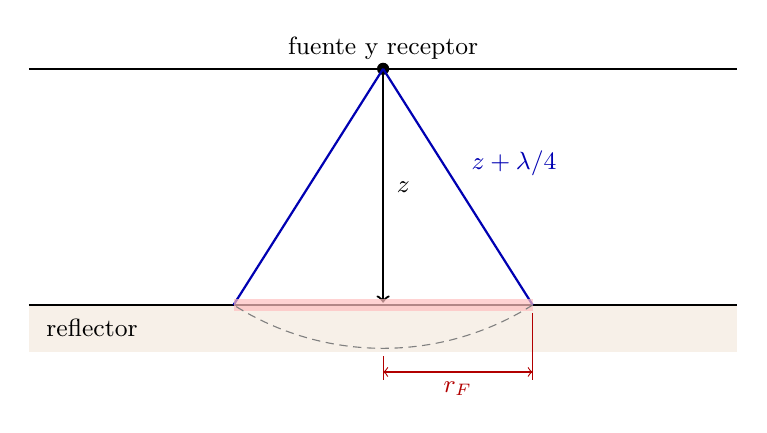
\begin{tikzpicture}[font=\small, x=1cm, y=1cm]
\fill[brown!12] (-4.5,-3.6) rectangle (4.5,-3.0);
\draw[thick] (-4.5,-3.0) -- (4.5,-3.0);
\node[anchor=north west] at (-4.4,-3.05) {reflector};
\draw[thick] (-4.5,0) -- (4.5,0);
\fill (0,0) circle (2.2pt) node[above] {fuente y receptor};
\draw[->, thick] (0,0) -- (0,-2.97);
\node[anchor=west] at (0.05,-1.5) {$z$};
\draw[blue!70!black, thick] (0,0) -- (1.9,-3.0);
\draw[blue!70!black, thick] (0,0) -- (-1.9,-3.0);
\node[anchor=west, blue!70!black] at (1.0,-1.2) {$z + \lambda/4$};
\fill[red!25, opacity=0.7] (-1.9,-3.08) rectangle (1.9,-2.92);
\draw[red!70!black] (0,-3.65) -- (0,-3.95) (1.9,-3.1) -- (1.9,-3.95);
\draw[<->, red!70!black] (0,-3.85) -- (1.9,-3.85) node[midway, below] {$r_F$};
\draw[gray, densely dashed] (-57.6:3.55) arc (-57.6:-122.4:3.55);
\end{tikzpicture}

\par\smallskip{\small La primera \omterm{def:b3:exploration-seismology:fresnel}{zona de Fresnel} (esquemática): la parte del
reflector cuya distancia a una fuente y un receptor coincidentes supera la
distancia normal $z$ en menos de $\lambda/4$ (arco discontinuo: la esfera de radio
$z + \lambda/4$), de modo que el exceso de camino de ida y vuelta es menor que media longitud de onda
y sus ecos llegan en fase. La escala de $\lambda$ está exagerada.}
\label{fig:b3:exploration-seismology:fresnel}
\end{omfigure}

\section{Adquisición y procesado de punto medio común}

Un eco aislado es demasiado débil para distinguirlo del ruido. Por ello, los
levantamientos de reflexión registran cada punto del subsuelo muchas veces, con
distintos pares fuente--receptor, y suman los registros.

\begin{definition}[Punto medio común, cobertura]\label{def:b3:exploration-seismology:cmp}
Para una fuente en $x_s$ y un receptor en $x_r$ sobre una línea, el punto medio es
$(x_s + x_r)/2$ y el desplazamiento $x = |x_r - x_s|$. Un conjunto de \emph{punto medio
común}\index{punto medio común} (CMP) es el conjunto de trazas, procedentes de todos
los disparos, que comparten el mismo punto medio; sobre capas planas, todas ellas
se reflejan en el mismo punto del subsuelo. La \emph{cobertura (sísmica)}\index{cobertura (sísmica)}
es el número de trazas de un conjunto. Con $N$ canales a la
separación de receptores $\Delta g$ y un disparo cada $\Delta s$ a lo largo de la línea, la
cobertura es $N\Delta g/(2\Delta s)$.
\end{definition}

\begin{omfigure}
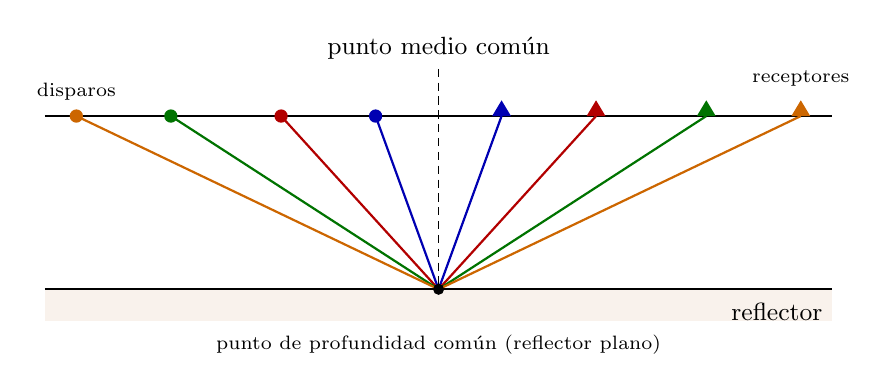
\begin{tikzpicture}[font=\small, x=1cm, y=1cm]
\draw[thick] (-5,0) -- (5,0);
\fill[brown!10] (-5,-2.6) rectangle (5,-2.2);
\draw[thick] (-5,-2.2) -- (5,-2.2);
\node[anchor=north east] at (5,-2.25) {reflector};
\foreach \off/\col in {0.8/blue!70!black, 2.0/red!70!black, 3.4/green!45!black, 4.6/orange!80!black} {
  \draw[\col, thick] (-\off,0) -- (0,-2.2) -- (\off,0);
  \fill[\col] (-\off,0) circle (2.4pt);
  \fill[\col] (\off-0.12,0) -- (\off+0.12,0) -- (\off,0.2) -- cycle;
}
\fill (0,-2.2) circle (2pt);
\draw[densely dashed] (0,0.6) -- (0,-2.2);
\node[anchor=south] at (0,0.6) {punto medio común};
\node[anchor=north, align=center, font=\scriptsize] at (0,-2.65) {punto de profundidad común (reflector plano)};
\node[anchor=south, font=\scriptsize] at (-4.6,0.08) {disparos};
\node[anchor=south, font=\scriptsize] at (4.6,0.25) {receptores};
\end{tikzpicture}

\par\smallskip{\small Geometría de \omterm{def:b3:exploration-seismology:cmp}{punto medio común} (esquemática): cuatro parejas fuente--receptor
(puntos, triángulos) de distinto desplazamiento comparten el mismo punto medio; sobre un
reflector plano, todas se reflejan en el mismo punto situado debajo de él. Sus trazas forman un
conjunto de cobertura cuatro.}
\label{fig:b3:exploration-seismology:cmp}
\end{omfigure}

\begin{theorem}[Sobretiempo normal]\label{thm:b3:exploration-seismology:nmo}
En una capa de velocidad $v$ situada sobre un reflector plano, a un tiempo vertical de ida
y vuelta $t_0$, la reflexión registrada a desplazamiento $x$ llega en
\[
  t(x)^2 = t_0^2 + \frac{x^2}{v^2},
\]
una hipérbola en el plano $(x, t)$. El retraso $\Delta t = t(x) - t_0$ es el
\emph{sobretiempo normal}\index{sobretiempo normal}; para $x \ll vt_0$,
$\Delta t \approx x^2/(2v^2t_0)$.
\end{theorem}

\begin{proof}
El camino de la reflexión va desde la fuente hasta el punto de reflexión bajo el
punto medio y de vuelta al receptor: dos tramos de longitud
$\sqrt{(vt_0/2)^2 + (x/2)^2}$. Así, $t = (2/v)\sqrt{(vt_0/2)^2 + (x/2)^2}$ y
$t^2 = t_0^2 + x^2/v^2$. Entonces $t - t_0 = (t^2 - t_0^2)/(t + t_0) \approx
x^2/(2v^2t_0)$.
\end{proof}

Sobre varias capas, el tiempo de reflexión ya no es exactamente hiperbólico, pero lo es
casi a desplazamientos pequeños, con una velocidad que es una media ponderada de las
de las capas.

\begin{definition}[Velocidades de apilamiento, cuadrática media y de intervalo]\label{def:b3:exploration-seismology:velocities}
La \emph{velocidad de intervalo}\index{velocidad de intervalo} $v_i$ de una capa es su
propia velocidad; con $\Delta t_i = 2h_i/v_i$ el tiempo de ida y vuelta a través de ella, la
\emph{velocidad cuadrática media}\index{velocidad cuadrática media} hasta la
base de la capa $n$ es
\[
  V_{\text{rms},n} = \left(\frac{\sum_{i\le n}v_i^2\,\Delta t_i}{\sum_{i\le n}\Delta t_i}\right)^{1/2}.
\]
La \emph{velocidad de apilamiento}\index{velocidad de apilamiento} de una reflexión es la
velocidad $V$ de la hipérbola $t^2 = t_0^2 + x^2/V^2$ que mejor ajusta sus tiempos en un
conjunto de \omterm{def:b3:exploration-seismology:cmp}{punto medio común}.
\end{definition}

\begin{proposition}[Velocidad de apilamiento a desplazamientos pequeños]\label{prop:b3:exploration-seismology:rms}
Sobre capas planas, $t(x)^2 = t_0^2 + x^2/V_{\text{rms}}^2 + O(x^4)$: a desplazamientos
pequeños, la \omterm{def:b3:exploration-seismology:velocities}{velocidad de apilamiento} es la \omterm{def:b3:exploration-seismology:velocities}{velocidad cuadrática media}.
\end{proposition}

\begin{proof}
Para el \omterm{def:b3:seismology-imaging:ray-parameter}{parámetro del rayo} $p$, $x = \sum_i 2h_i\tan\varphi_i$ y
$t = \sum_i 2h_i/(v_i\cos\varphi_i)$, con $\sin\varphi_i = pv_i$. Hasta segundo
orden en $p$, $\tan\varphi_i \approx pv_i$ y $1/\cos\varphi_i \approx 1 +
p^2v_i^2/2$, así que $x \approx p\sum v_i^2\Delta t_i = pV_{\text{rms}}^2t_0$ y
$t \approx t_0 + \tfrac12p^2V_{\text{rms}}^2t_0$. Entonces
$t^2 \approx t_0^2 + p^2V_{\text{rms}}^2t_0^2 = t_0^2 + x^2/V_{\text{rms}}^2$, siendo los términos
despreciados de orden $p^4$, es decir, $x^4$.
\end{proof}

\begin{theorem}[Ecuación de Dix]\label{thm:b3:exploration-seismology:dix}
Si $V_{n-1}$ y $V_n$ son las \omterm{def:b3:exploration-seismology:velocities}{velocidades cuadráticas medias} hasta el techo y la base de la capa
$n$, a los tiempos de ida y vuelta $t_{n-1}$ y $t_n$, la \omterm{def:b3:exploration-seismology:velocities}{velocidad de intervalo} de la
capa viene dada por la \emph{ecuación de Dix}\index{ecuación de Dix}
\[
  v_n^2 = \frac{V_n^2t_n - V_{n-1}^2t_{n-1}}{t_n - t_{n-1}} ,
\]
y su espesor es $h_n = v_n(t_n - t_{n-1})/2$.
\end{theorem}

\begin{proof}
Por definición $V_n^2t_n = \sum_{i\le n}v_i^2\Delta t_i$ y $V_{n-1}^2t_{n-1}
= \sum_{i\le n-1}v_i^2\Delta t_i$. Su diferencia es $v_n^2\Delta t_n$, con
$\Delta t_n = t_n - t_{n-1}$.
\end{proof}

El análisis de velocidades recorre cada conjunto en busca de la hipérbola que mejor se ajusta a la
energía: para cada $t_0$ y $V$ de prueba, las trazas se suman a lo largo de la curva, y
se representa una medida de coherencia (la semblanza); el analista escoge sus máximos,
reflector a reflector, para construir una función de velocidades. La corrección de \omterm{thm:b3:exploration-seismology:nmo}{sobretiempo normal}
desplaza cada muestra de cada traza desde $t(x)$ hasta $t_0$, aplanando las
reflexiones, y las trazas de cada conjunto se suman.

\begin{definition}[Apilamiento (sísmico)]\label{def:b3:exploration-seismology:stack}
El \emph{apilamiento (sísmico)}\index{apilamiento (sísmico)} es la suma, tras la
corrección de \omterm{thm:b3:exploration-seismology:nmo}{sobretiempo normal}, de las trazas de un conjunto de \omterm{def:b3:exploration-seismology:cmp}{punto medio común} en una única traza
situada en el punto medio. Las trazas apiladas, dispuestas una junto a otra a lo largo de la línea, forman
la sección apilada, una imagen de los reflectores en tiempo de ida y vuelta.
\end{definition}

\begin{proposition}[Ganancia de un apilamiento]\label{prop:b3:exploration-seismology:sqrtN}
Si las $N$ trazas de un conjunto llevan la misma señal de reflexión y un ruido independiente
de igual desviación típica $\sigma$, su media lleva la misma señal y un ruido
de desviación típica $\sigma/\sqrt N$: el apilamiento eleva la
relación señal-ruido en $\sqrt N$.
\end{proposition}

\begin{proof}
La varianza de una suma de $N$ variables independientes es la suma de sus
varianzas, $N\sigma^2$; dividida entre $N^2$, la media tiene la varianza
$\sigma^2/N$ (la desviación típica de la media, recordada de los libros de
matemáticas).
\end{proof}

\begin{omfigure}
\begin{tikzpicture}
\begin{groupplot}[group style={group size=2 by 1, horizontal sep=0.5cm, y descriptions at=edge left},
  width=0.52\linewidth, height=0.56\linewidth, y dir=reverse, ymin=0.4, ymax=0.92,
  xmin=-150, xmax=2150, tick label style={font=\scriptsize}, title style={font=\small},
  xlabel={\scriptsize desplazamiento (\unit{m})}]
\nextgroupplot[title={(a) Conjunto CMP}, ylabel={tiempo de ida y vuelta (\unit{s})}]
\addplot[black, very thin, unbounded coords=jump] table[x=x, y=t] {figdata/out/bachelor-3-cmp_nmo-gather-raw.dat};
\nextgroupplot[title={(b) tras la corrección de sobretiempo normal}]
\addplot[black, very thin, unbounded coords=jump] table[x=x, y=t] {figdata/out/bachelor-3-cmp_nmo-gather-nmo.dat};
\end{groupplot}
\end{tikzpicture}

\par\smallskip{\small Conjunto CMP sintético bajo el eje del sinclinal de la
línea Varden (calculado por trazado exacto de rayos a través de la columna de
capas planas; \omterm{def:b3:exploration-seismology:wavelet}{ondícula de Ricker} de 30 Hz; sin ruido). (a) Las cuatro
reflexiones (techo de la lutita, techo y base de la caliza, techo del
basamento) se curvan hacia abajo al aumentar el desplazamiento, siguiendo
hipérbolas casi perfectas. (b) Tras la corrección de \omterm{thm:b3:exploration-seismology:nmo}{sobretiempo normal} con las
\omterm{def:b3:exploration-seismology:velocities}{velocidades de apilamiento} ajustadas a los desplazamientos hasta \qty{600}{m},
las reflexiones son planas hasta unos \qty{1}{km}; más allá, los tiempos
verdaderos se apartan de la hipérbola, la corrección los deja curvados y las
ondículas se estiran; en el procesado, las trazas lejanas estiradas de las reflexiones someras se silencian antes del apilamiento.}
\label{fig:b3:exploration-seismology:gather}
\end{omfigure}

\begin{omfigure}
\begin{tikzpicture}
\begin{axis}[omrecord, width=0.72\linewidth, height=0.46\linewidth,
  xmin=0.4, xmax=0.78, ymin=2000, ymax=5000,
  xlabel={tiempo de ida y vuelta $t_0$ (\unit{s})}, ylabel={velocidad (\unit{m.s^{-1}})},
  legend cell align=left, legend columns=2,
  legend style={font=\scriptsize, at={(0.5,-0.24)}, anchor=north}]
\addplot[gray, thick, const plot mark right] table[x=t0, y=vint] {figdata/out/bachelor-3-cmp_nmo-vel.dat};
\addlegendentry{velocidad de intervalo del modelo}
\addplot[gray, thick, forget plot] coordinates {(0.4,2500) (0.487847,2500)};
\addplot[blue!70!black, thick, mark=*, mark size=1.5pt] table[x=t0, y=vrms] {figdata/out/bachelor-3-cmp_nmo-vel.dat};
\addlegendentry{velocidad cuadrática media}
\addplot[red!70!black, only marks, mark=square*, mark size=1.6pt] table[x=t0, y=vstack] {figdata/out/bachelor-3-cmp_nmo-vel.dat};
\addlegendentry{velocidad de apilamiento (desplazamientos hasta \qty{600}{m})}
\addplot[green!45!black, only marks, mark=triangle*, mark size=2pt] table[x=t0, y=vdix] {figdata/out/bachelor-3-cmp_nmo-vel.dat};
\addlegendentry{velocidad de intervalo de Dix}
\end{axis}
\end{tikzpicture}

\par\smallskip{\small Velocidades bajo el eje del sinclinal (calculadas). La \omterm{def:b3:exploration-seismology:velocities}{velocidad cuadrática media},
una media ponderada, cambia lentamente; las \omterm{def:b3:exploration-seismology:velocities}{velocidades de apilamiento} del conjunto se sitúan
cerca de ella. Aplicada a ellas, la \omterm{thm:b3:exploration-seismology:dix}{ecuación de Dix} recupera la \omterm{def:b3:exploration-seismology:velocities}{velocidad de intervalo} de cada capa
(la línea escalonada, trazada en la base de cada capa) con un error de unos
pocos por ciento, que crece en la caliza delgada y rápida.}
\label{fig:b3:exploration-seismology:velocities}
\end{omfigure}

\begin{omfigure}
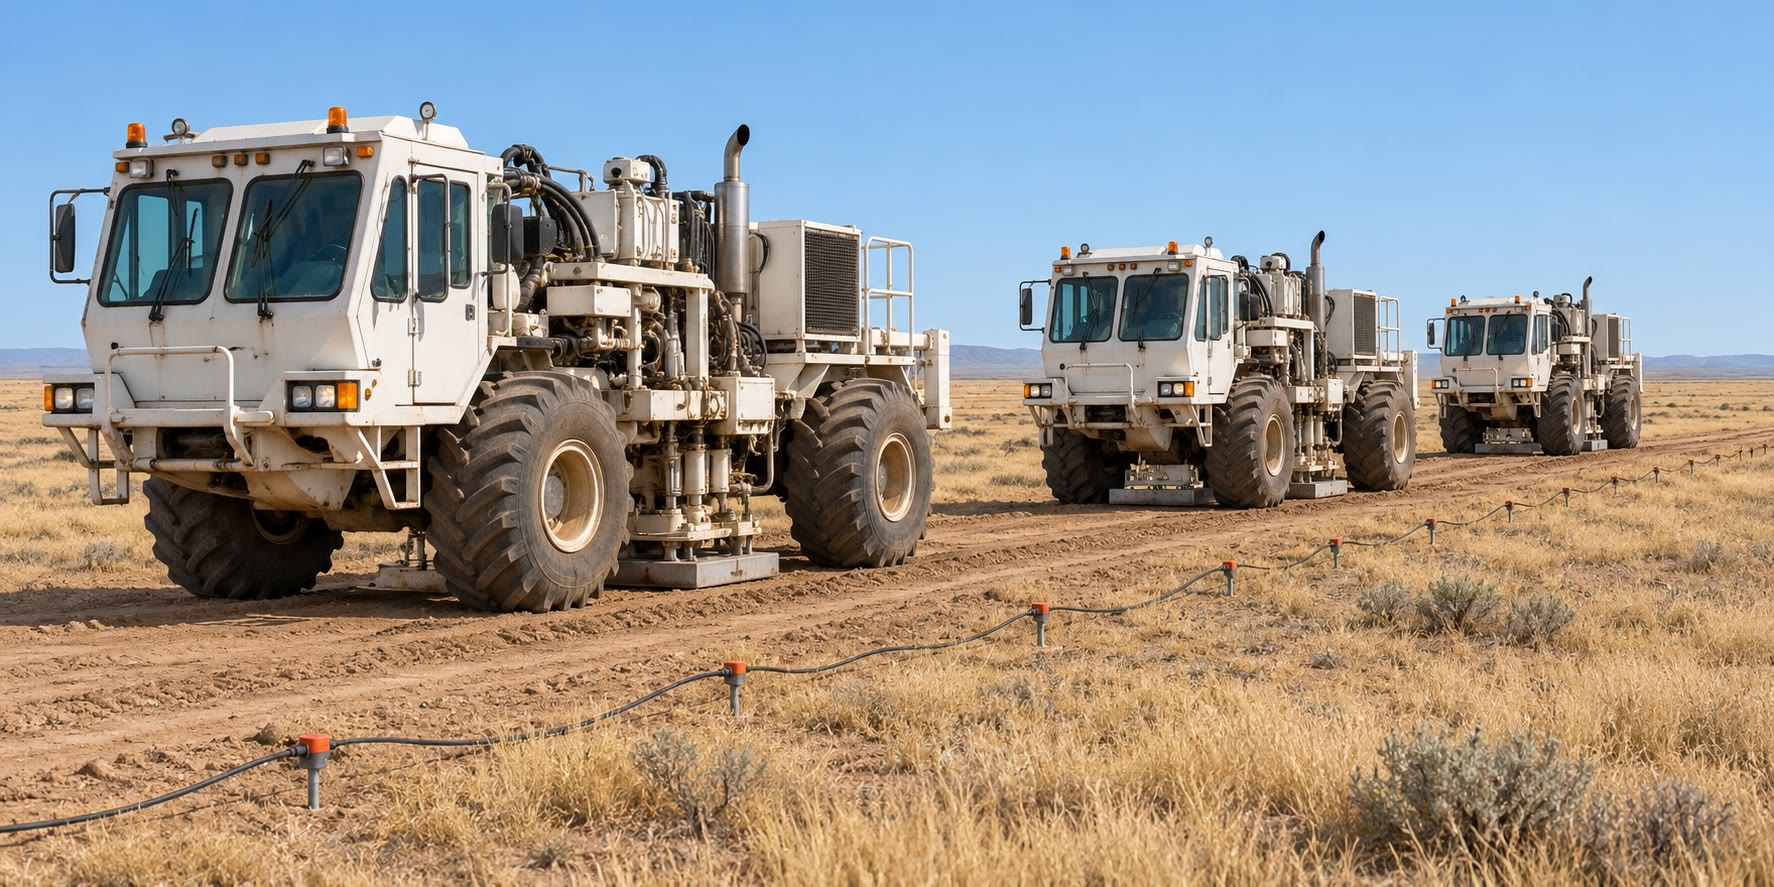
\includegraphics[width=0.62\linewidth]{images/book5/ai/b3-vibroseis.jpg}

\par\smallskip{\small Camiones vibradores en una línea de prospección terrestre: en lugar de una explosión,
cada camión apoya una placa pesada sobre el suelo y la hace vibrar con un barrido de frecuencias durante varios segundos;
los registros largos se comprimen en pulsos breves al correlacionarlos con el barrido
(Ilustración generada por IA.)}
\label{fig:b3:exploration-seismology:vibroseis}
\end{omfigure}

\section{Migración}

Una sección apilada muestra cada reflexión bajo el punto medio donde se
registró, en el tiempo que tardó en volver. Para un reflector horizontal ahí
está. Para uno buzante no: el eco registrado en un punto de la superficie
procede del punto del reflector más cercano a él, que se halla hacia arriba
del buzamiento, no verticalmente debajo. Puntos como los cortes de falla, que
dispersan energía en todas las direcciones, aparecen como hipérbolas.

\begin{definition}[Migración sísmica]\label{def:b3:exploration-seismology:migration}
La \emph{migración sísmica}\index{migración sísmica} es la etapa de
procesado que traslada las reflexiones de una sección sísmica a las posiciones
de los reflectores que las produjeron: restaura los buzamientos verdaderos y las
posiciones de los reflectores buzantes y colapsa las hipérbolas de difracción de
los dispersores puntuales sobre sus vértices. Realizada con un modelo de
velocidades en tiempo, proporciona una sección migrada en tiempo; con un modelo en profundidad, una imagen en profundidad.
\end{definition}

\begin{theorem}[Buzamiento en una sección de desfase cero]\label{thm:b3:exploration-seismology:dip}
En un medio de velocidad $v$, un reflector plano de buzamiento $\theta$ en el
plano de la sección aparece en la sección de desfase cero, representada como la
profundidad $vt/2$ verticalmente debajo de cada punto de registro, como una
línea de buzamiento aparente $\theta_a$ con
\[
  \tan\theta_a = \sin\theta .
\]
La reflexión registrada en el punto $x$ procede del punto del reflector situado a
una distancia $(vt/2)\sin\theta$ hacia arriba del buzamiento, respecto del punto situado verticalmente debajo de $x$.
\end{theorem}

\begin{proof}
El rayo de desfase cero es normal al reflector, de modo que el tiempo registrado
en $x$ es $t = 2d(x)/v$, donde $d(x)$ es la distancia de $x$ al plano. Esa
distancia crece en $\sin\theta$ por cada unidad de $x$ en la dirección del
buzamiento, así que la profundidad representada $vt/2 = d(x)$ tiene la
pendiente $\sin\theta$. El pie de la normal desde $x$ al plano se encuentra a
la distancia horizontal $d\sin\theta$ de $x$, en el lado hacia arriba del buzamiento.
\end{proof}

Puesto que $\tan\theta_a = \sin\theta < \tan\theta$, una sección sin migrar muestra siempre
buzamientos más suaves que los verdaderos, y no puede mostrar buzamientos más empinados que \ang{45}. Un dispersor puntual a profundidad $z$
bajo el punto $x_0$ devuelve en $x$ el tiempo de desfase cero
$t(x) = (2/v)\sqrt{z^2 + (x - x_0)^2}$: una hipérbola con su vértice sobre el
punto, la difracción. La migración en su forma más simple, la apilación de
difracciones, suma cada sección a lo largo de la hipérbola de difracción de
cada dispersor posible y deposita la suma en el vértice: los reflectores, que
son líneas continuas de dispersores, emergen en sus lugares verdaderos, y las
difracciones se colapsan.

\begin{omfigure}
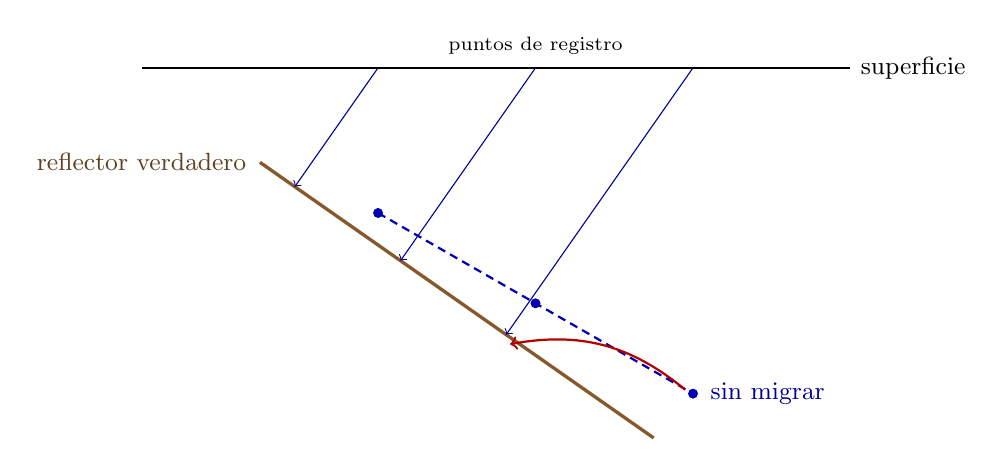
\begin{tikzpicture}[font=\small, x=1cm, y=1cm]
\draw[thick] (-0.5,0) -- (8.5,0) node[right] {superficie};
% true reflector, dip 35 deg, rising to the left
\draw[very thick, brown!70!black] (1.0,-1.2) -- (6.0,-4.70);
\node[brown!50!black, anchor=east] at (0.95,-1.2) {reflector verdadero};
% zero-offset normal rays from x = 2, 4, 6
\foreach \x in {2.5, 4.5, 6.5} {
  % distance from (x,0) to the line through (1,-1.2) dir (cos35,-sin35): normal n=(sin35,cos35)
  \pgfmathsetmacro{\dd}{abs(0.5736*(\x-1.0) + 0.8192*(0+1.2))}
  \draw[blue!60!black, ->] (\x,0) -- ++({-0.5736*\dd},{-0.8192*\dd});
  \fill[blue!70!black] (\x,{-\dd}) circle (1.8pt);
}
% apparent reflector through the plotted points
\pgfmathsetmacro{\da}{abs(0.5736*1.5 + 0.8192*1.2)}
\pgfmathsetmacro{\db}{abs(0.5736*5.5 + 0.8192*1.2)}
\draw[blue!70!black, thick, densely dashed] (2.5,{-\da}) -- (6.5,{-\db});
\node[blue!60!black, anchor=west] at (6.6,{-\db}) {sin migrar};
\node[anchor=south, font=\scriptsize] at (4.5,0.05) {puntos de registro};
\draw[->, red!70!black, thick] (6.4,{-\db+0.05}) to[bend right=25] ({6.5-0.5736*\db+0.05},{-0.8192*\db-0.12});
\end{tikzpicture}

\par\smallskip{\small Migración de un reflector buzante (esquema, buzamiento
verdadero \ang{35}). El rayo de desfase cero en cada punto de registro es
normal al reflector, de modo que su eco procede de la parte alta del buzamiento; representado verticalmente bajo el punto,
a la profundidad $vt/2$, el reflejo aparece más suave (en trazos: $\tan\theta_a =
\sin\theta$, aquí \ang{29.8}), y desplazado hacia la parte baja del buzamiento. La migración (flecha roja) lo devuelve a su lugar.}
\label{fig:b3:exploration-seismology:migration}
\end{omfigure}

\section{Estratigrafía sísmica}

Una sección migrada es una imagen de la estratificación, y puede leerse como
estratigrafía: las reflexiones siguen las superficies de estratificación, que
son líneas de tiempo, de modo que su geometría registra cómo se llenó la cuenca.

\begin{definition}[Estratigrafía sísmica, facies sísmicas]\label{def:b3:exploration-seismology:seismic-stratigraphy}
La \emph{estratigrafía sísmica}\index{estratigrafía sísmica} es la interpretación
de la estratigrafía y de la historia deposicional de una cuenca a partir de la
geometría de sus reflexiones sísmicas. Una \emph{facies sísmica}\index{facies sísmica} es una
unidad tridimensional de reflexiones cuyo carácter (continuidad, amplitud,
frecuencia, geometría interna: paralela, divergente, sigmoidal, caótica, abombada)
difiere del de sus vecinas y se interpreta como un
ambiente de depósito.
\end{definition}

\begin{definition}[Terminaciones de reflectores]\label{def:b3:exploration-seismology:terminations}
Una \emph{terminación de reflector}\index{terminación de reflector} es el final de una
reflexión contra otra. \emph{Onlap}\index{onlap}: una reflexión inicialmente horizontal
termina contra una superficie que asciende con mayor pendiente, de modo que los
estratos más jóvenes se apoyan sobre una pendiente antigua. \emph{Downlap}\index{downlap}: una reflexión inclinada
termina, hacia la parte baja del buzamiento, contra una superficie más suave, tal como
ocurre cuando los pies de los estratos progradantes descansan sobre el fondo de una cuenca. \emph{Toplap}\index{toplap}: las
reflexiones inclinadas terminan, hacia la parte alta del buzamiento, contra una superficie suprayacente, con poca erosión, como
ocurre cuando los topes de los estratos progradantes alcanzan el nivel del mar. \emph{Truncación
erosiva}\index{truncación erosiva}: las reflexiones terminan, hacia la parte alta del buzamiento, contra una
superficie suprayacente que las corta, una discordancia.
\end{definition}

\begin{omfigure}
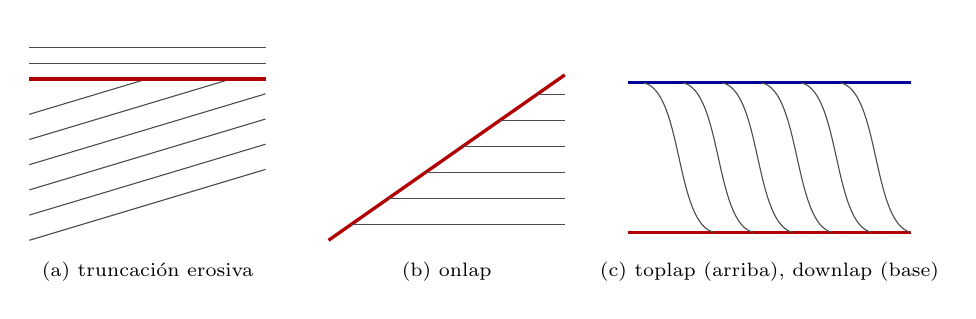
\begin{tikzpicture}[font=\scriptsize, x=1cm, y=1cm]
% erosional truncation: tilted beds cut by an unconformity
\begin{scope}
\foreach \k in {0,...,5} {\draw[gray!60!black] (0,{-2.3+0.32*\k}) -- (3.0,{-1.4+0.32*\k-0.25*0});}
\fill[white] (0,-0.25) -- (3.2,-0.25) -- (3.2,0.4) -- (0,0.4) -- cycle;
\draw[very thick, red!70!black] (0,-0.25) -- (3.0,-0.25);
\foreach \k in {0,1} {\draw[gray!60!black] (0,{-0.05+0.2*\k}) -- (3.0,{-0.05+0.2*\k});}
\node[anchor=north] at (1.5,-2.45) {(a) truncación erosiva};
\end{scope}
% onlap
\begin{scope}[xshift=3.8cm]
\draw[very thick, red!70!black] (0,-2.3) -- (3.0,-0.2);
\foreach \k in {0,...,5} {\pgfmathsetmacro{\y}{-2.1+0.33*\k} \pgfmathsetmacro{\xe}{(\y+2.3)/0.7} \draw[gray!60!black] (\xe,\y) -- (3.0,\y);}
\node[anchor=north] at (1.5,-2.45) {(b) onlap};
\end{scope}
% downlap and toplap: clinoforms
\begin{scope}[xshift=7.6cm]
\draw[very thick, red!70!black] (0,-2.2) -- (3.6,-2.2);
\draw[very thick, blue!60!black] (0,-0.3) -- (3.6,-0.3);
\foreach \k in {0,...,5} {\draw[gray!60!black] ({0.2+0.5*\k},-0.3) .. controls ({0.7+0.5*\k},-0.4) and ({0.6+0.5*\k},-2.1) .. ({1.1+0.5*\k},-2.2);}
\node[anchor=north] at (1.8,-2.45) {(c) toplap (arriba), downlap (base)};
\end{scope}
\end{tikzpicture}

\par\smallskip{\small Terminaciones de reflectores (secciones esquemáticas, reflexiones en gris,
superficies terminales en color). (a) Reflexiones inclinadas cortadas por una
discordancia. (b) Reflexiones horizontales que terminan contra una pendiente antigua. (c) Estratos
inclinados de una cuña progradante que terminan hacia la parte alta del buzamiento contra la superficie superior (\omterm{def:b3:exploration-seismology:terminations}{toplap}) y
hacia la parte baja, sobre el fondo de la cuenca (\omterm{def:b3:exploration-seismology:terminations}{downlap}).}
\label{fig:b3:exploration-seismology:terminations}
\end{omfigure}

Las terminaciones marcan las superficies que delimitan secuencias de estratos
genéticamente relacionados; cartografiarlas en una cuenca y relacionarlas con el
ascenso y descenso del nivel relativo del mar, es la estratigrafía secuencial, materia del
\cref{ch:b3:sequence-stratigraphy}. Una sección sísmica de un margen pasivo
muestra típicamente cuñas de reflexiones progradantes hacia el mar que se apoyan (\omterm{def:b3:exploration-seismology:terminations}{downlap}) sobre el
fondo profundo, coronadas por \omterm{def:b3:exploration-seismology:terminations}{toplap}, y quedan sepultadas hacia tierra bajo estratos en \omterm{def:b3:exploration-seismology:terminations}{onlap} depositados
cuando el mar volvió a subir.

\begin{inthefield}[Un tendido sísmico marino y una cuadrilla en tierra]
\begin{minipage}[t]{0.55\linewidth}\vspace{0pt}
En un levantamiento marino el buque nunca se detiene: navega línea tras línea a
unos nudos, disparando las matrices de cañones de aire a intervalos fijos, y los cables remolcados mantenidos a
profundidad constante mediante pequeñas alas orientables y localizados por posicionamiento
acústico y por satélite. Los observadores en el puente vigilan el mar alrededor de la matriz, y el
levantamiento se rige por normas que establecen las medidas para proteger a los mamíferos marinos,
la guardia que se mantiene y lo que se informa.
% ledger: noaa5:itr-gom
En tierra, la cuadrilla tiende cables o unidades de registro inalámbricas a lo largo de las líneas;
los camiones vibradores avanzan en convoy de un punto fuente al siguiente, y un
camión de registro comprueba cada canal antes de cada barrido. De vuelta en el centro de procesado,
los registros se ordenan en colecciones de \omterm{def:b3:exploration-seismology:cmp}{punto medio común}, se escogen las velocidades,
los datos se apilan y migran, y la sección se entrega a los
intérpretes.
\end{minipage}\hfill
\begin{minipage}[t]{0.42\linewidth}\vspace{0pt}
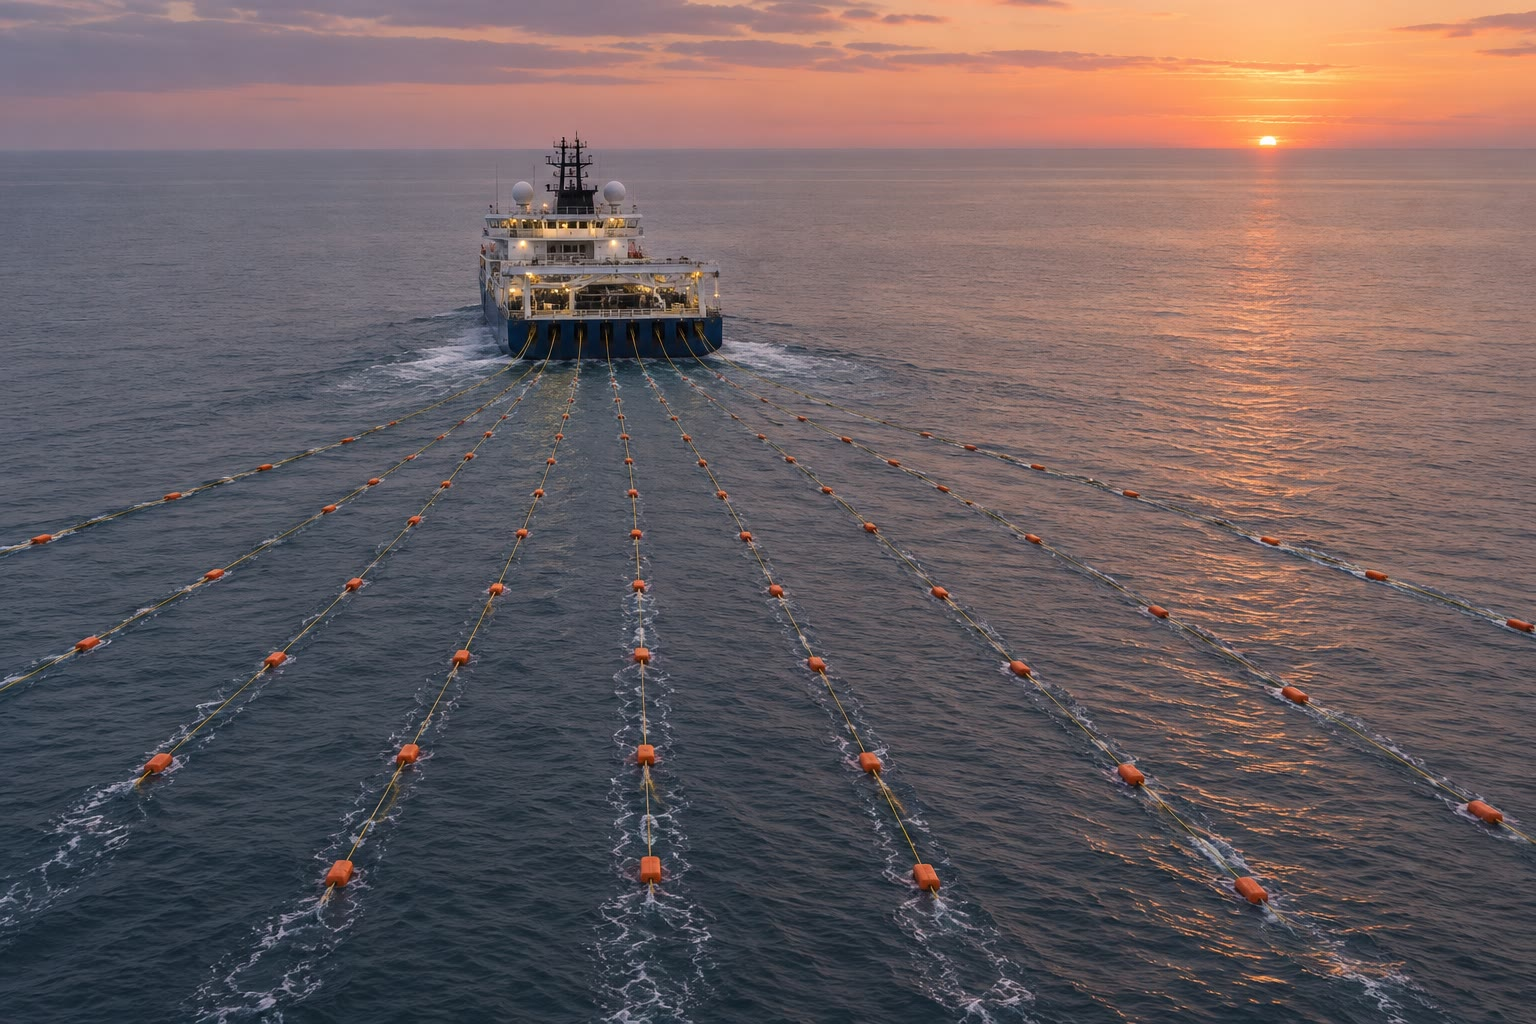
\includegraphics[width=\linewidth]{images/book5/ai/b3-streamer-vessel.jpg}

{\scriptsize Un buque de prospección sísmica que remolca sus cables al atardecer
(Ilustración generada por IA.)}
\end{minipage}
\end{inthefield}

\section{Ejercicios}

\begin{exercise}[$\star$]\label{exo:b3:exploration-seismology:1}
La creta ($v = \qty{2500}{m.s^{-1}}$, $\rho = \qty{2.00}{g.cm^{-3}}$) yace sobre lutita
(\qty{2300}{m.s^{-1}}, \qty{2.30}{g.cm^{-3}}), que a su vez yace sobre caliza
(\qty{4500}{m.s^{-1}}, \qty{2.60}{g.cm^{-3}}). Calcúlense las tres impedancias y los
coeficientes de reflexión de las dos interfases. ¿Qué fracción de la energía incidente
refleja la parte superior de la caliza?
% ledger: mavko:velocities
\end{exercise}

\begin{exercise}[$\star$]\label{exo:b3:exploration-seismology:2}
Un reflector plano yace a \qty{800}{m} por debajo de una capa de \qty{2000}{m.s^{-1}}.
Calcúlense $t_0$, el tiempo de reflexión a un desplazamiento de \qty{1000}{m}, y el
\omterm{thm:b3:exploration-seismology:nmo}{sobretiempo normal} allí. Compárese con la aproximación $x^2/(2v^2t_0)$.
\end{exercise}

\begin{exercise}[$\star$]\label{exo:b3:exploration-seismology:3}
Un cable sísmico tiene 240 canales separados \qty{12.5}{m}, y el buque dispara cada
\qty{25}{m}. Calcúlense el intervalo de \omterm{def:b3:exploration-seismology:cmp}{punto medio común} y la cobertura. ¿Qué intervalo
entre disparos daría una cobertura de 120?
\end{exercise}

\begin{exercise}[$\star$]\label{exo:b3:exploration-seismology:4}
Con una frecuencia dominante de \qty{30}{Hz}, calcúlense la longitud de onda y el
cuarto de longitud de onda en arenisca de \qty{3000}{m.s^{-1}} y en caliza de
\qty{4500}{m.s^{-1}}. Calcúlese el radio de la primera \omterm{def:b3:exploration-seismology:fresnel}{zona de Fresnel} de un
reflector situado a \qty{1000}{m} de profundidad bajo rocas de velocidad media de \qty{2800}{m.s^{-1}}.
\end{exercise}

\begin{exercise}[$\star\star$]\label{exo:b3:exploration-seismology:5}
Dos reflexiones tienen $t_0 = \qty{0.500}{s}$ con una \omterm{def:b3:exploration-seismology:velocities}{velocidad cuadrática media} de
\qty{2400}{m.s^{-1}}, y $t_0 = \qty{0.700}{s}$ con \qty{2800}{m.s^{-1}}.
Calcúlense la \omterm{def:b3:exploration-seismology:velocities}{velocidad de intervalo} y el espesor de la capa comprendida entre ellas.
\end{exercise}

\begin{exercise}[$\star\star$]\label{exo:b3:exploration-seismology:6}
Un reflector plano buza un ángulo $\varphi$ en el plano de una línea de \omterm{def:b3:exploration-seismology:cmp}{punto medio común}, en una capa de
velocidad $v$. (a) Demuéstrese que $t(x)^2 = t_0^2 + x^2\cos^2\varphi/v^2$, donde $t_0$ es
el tiempo de desplazamiento nulo en el punto medio. (Indicación: utilícese la imagen del punto medio en
el reflector.) (b) Dedúzcase la \omterm{def:b3:exploration-seismology:velocities}{velocidad de apilamiento} y calcúlese para
$v = \qty{2000}{m.s^{-1}}$ y $\varphi = \ang{12}$.
\end{exercise}

\begin{exercise}[$\star\star$]\label{exo:b3:exploration-seismology:7}
Una colección de cobertura 60 tiene ruido independiente de igual varianza en cada traza. ¿En
qué factor eleva el apilamiento la relación señal-ruido? ¿En qué factor
debe aumentarse la cobertura para duplicarla de nuevo?
\end{exercise}

\begin{exercise}[$\star\star$]\label{exo:b3:exploration-seismology:8}
En una sección de tiempos de desplazamiento nulo, en roca de \qty{3000}{m.s^{-1}}, una reflexión
asciende \qty{0.40}{s} de tiempo de ida y vuelta por kilómetro a lo largo de la línea. Conviértase esta
pendiente en un buzamiento aparente, y calcúlese el buzamiento real del reflector.
\end{exercise}

\begin{exercise}[$\star\star$]\label{exo:b3:exploration-seismology:9}
Calcúlese la convolución de la \omterm{def:b3:exploration-seismology:synthetic}{serie de reflectividad} $r = (0, 0.3, 0, -0.2, 0)$ con la
ondícula de tres muestras $w = (-0.5, 1, -0.5)$, muestra a muestra. ¿Dónde están las dos
reflexiones y se solapan entre sí?
\end{exercise}

\begin{exercise}[$\star\star\star$]\label{exo:b3:exploration-seismology:10}
Un perfil de refracción inverso sobre una capa de \qty{1800}{m.s^{-1}} da una
velocidad aparente hacia el buzamiento de \qty{2900}{m.s^{-1}} y otra contra el buzamiento de
\qty{4400}{m.s^{-1}}. Calcúlense el ángulo crítico, el buzamiento y la velocidad del
refractor. Compárese la velocidad del refractor con la media armónica de las dos
velocidades aparentes.
\end{exercise}

\begin{exercise}[$\star\star\star$]\label{exo:b3:exploration-seismology:11}
En la \cref{prop:b3:exploration-seismology:tuning}, un estrato tiene coeficientes de reflexión
$+R$ y $-R$. (a) Demuéstrese que, para $\Delta t \ll T$, la señal compuesta
es aproximadamente $R\,\Delta t\,w'(t)$, la derivada temporal de la ondícula
escalada por el espesor de ida y vuelta del estrato. (b) Explíquese por qué un estrato delgado todavía puede
detectarse, aunque no resuelto, y cómo podría estimarse su espesor a partir de
su amplitud. (c) Dos estratos de la misma roca, de 5 y \qty{10}{m} de espesor, se
obtienen imágenes con la misma ondícula: ¿cuál es la razón de sus amplitudes?
\end{exercise}

\begin{exercise}[$\star\star\star$]\label{exo:b3:exploration-seismology:12}
Un dispersor puntual yace a \qty{600}{m} por debajo de la línea, en roca de
\qty{3000}{m.s^{-1}}. (a) Escríbase el tiempo de desplazamiento nulo de su difracción en función de
la distancia horizontal $x$ al punto situado encima, y calcúlese para $x = 0$
y \qty{300}{m}. (b) Demuéstrese que la difracción es una hipérbola de la forma del
\omterm{thm:b3:exploration-seismology:nmo}{sobretiempo normal} con la velocidad $v/2$, y explíquese por qué una difracción es siempre más curvada que una
reflexión con el mismo tiempo en el vértice. (c) ¿Qué efecto tiene la migración sobre ella?
\end{exercise}

\section{Problema: una línea sísmica a través de las colinas de Varden}

\begin{problem}[{Problema de fin de semana --- refracción, análisis de velocidades, conversión a
profundidad y migración a lo largo de la sección A--B de las colinas de Varden}]
\label{pb:b3:exploration-seismology:1}
% values: calc/ch02.py, from figdata seismic_model.py, refraction_dip.py, cmp_nmo.py
Se adquiere una línea sísmica a lo largo de la sección A--B de las colinas de Varden, la región de
los mapas geológicos de los volúmenes anteriores. Sus distancias $s$ se cuentan desde
A a lo largo de la línea. La cobertera, de arriba abajo, está formada por creta, lutita (\qty{100}{m}),
caliza (\qty{180}{m}) y arenisca (\qty{120}{m}), que descansa discordantemente sobre
un basamento de esquistos; está plegada en un anticlinal y un sinclinal y cortada por una
falla normal.

\medskip
\noindent\textbf{Parte I --- Un tendido de refracción en el flanco O.} Un tendido de
\qty{1200}{m} se extiende entre los puntos de disparo O ($s = \qty{300}{m}$) y E
($s = \qty{1500}{m}$), sobre un terreno considerado horizontal. La creta y la lutita por encima de la
caliza se tratan como una única capa de $v_1 = \qty{2.40}{km.s^{-1}}$. Los
tiempos de onda de cabeza leídos en los registros son, desde O hacia E, \qty{425.2}{ms} a
\qty{800}{m} y \qty{486.1}{ms} a \qty{1200}{m}; desde E hacia O,
\qty{372.4}{ms} a \qty{800}{m} y \qty{486.1}{ms} a \qty{1200}{m}.
\begin{enumerate}
  \item Calcúlense las dos velocidades aparentes. ¿Cuál de los disparos está contra el buzamiento?
  \item Calcúlense el ángulo crítico y el buzamiento del refractor.
  \item Calcúlese la velocidad del refractor. ¿De qué roca se trata?
  \item Calcúlense los tiempos de intercepción y las profundidades perpendiculares del
        refractor bajo O y bajo E.
  \item Conviértanse en profundidades verticales y compruébese el buzamiento a partir de las dos profundidades.
  \item La lutita bajo la creta es más lenta que la creta. ¿Qué interpreta de ella la
        \omterm{def:b3:exploration-seismology:surveys}{prospección sísmica de refracción}, y cómo sesga las profundidades?
\end{enumerate}

\noindent\textbf{Parte II --- Análisis de velocidades en el PMC S.} Más al este, el PMC S
está sobre el eje del sinclinal, en el bloque hundido de la falla, donde
se supone que las capas son horizontales. Se toman cuatro reflexiones a separación cero y a
\qty{600}{m}:
\begin{center}
\small
\begin{tabular}{lcccc}
\hline
reflexión & 1 & 2 & 3 & 4 \\
$t_0$ (\unit{s}) & 0.4878 & 0.5748 & 0.6548 & 0.7348 \\
$t(\qty{600}{m})$ (\unit{s}) & 0.5437 & 0.6240 & 0.6887 & 0.7648 \\
\hline
\end{tabular}
\end{center}
\begin{enumerate}[resume]
  \item Calcúlese la velocidad NMO $V = x/\sqrt{t^2 - t_0^2}$ de las reflexiones 1
        y 2. ¿Por qué la segunda es menor que la primera?
  \item Calcúlese para las reflexiones 3 y 4.
  \item Tomándolas como \omterm{def:b3:exploration-seismology:velocities}{velocidades cuadráticas medias}, calcúlese la \omterm{def:b3:exploration-seismology:velocities}{velocidad de intervalo} de cada
        capa mediante la \omterm{thm:b3:exploration-seismology:dix}{ecuación de Dix}.
  \item Identifíquense las capas a partir de sus velocidades, y nómbrense las cuatro
        superficies reflectoras.
  \item La reflexión 1 es la más débil en los registros. ¿Por qué?
  \item ¿Por qué se midieron las velocidades solo en las separaciones de hasta \qty{600}{m}
        cuando el tendido alcanza \qty{2}{km}?
\end{enumerate}

\noindent\textbf{Parte III --- Conversión a profundidad y resolución.}
\begin{enumerate}[resume]
  \item Calcúlese el tiempo de ida y vuelta empleado en cada capa y su espesor.
  \item Calcúlese la profundidad de cada superficie reflectora bajo el terreno. Compárense
        los espesores de la lutita, la caliza y la arenisca con los valores
        dados anteriormente.
  \item Calcúlese la velocidad media desde el terreno hasta el basamento, y explíquese por qué
        la velocidad NMO de la reflexión 4 sobrestimaría la profundidad si se usara
        en su lugar.
  \item La ondícula de la prospección tiene su máximo en \qty{30}{Hz}. Calcúlese la longitud de onda en
        la lutita y su \omterm{def:b3:exploration-seismology:resolution}{espesor de sintonía}, tanto por la regla del cuarto de longitud de onda
        como mediante $b = v/(5.2f)$ para una \omterm{def:b3:exploration-seismology:wavelet}{ondícula de Ricker}. ¿Está resuelta la lutita?
        ¿A qué frecuencia entraría en sintonía por la regla del cuarto de longitud de onda?
  \item Calcúlese el radio de la primera \omterm{def:b3:exploration-seismology:fresnel}{zona de Fresnel} sobre el basamento, tomando
        $\lambda$ a partir de la velocidad NMO de la reflexión 4.
\end{enumerate}

\noindent\textbf{Parte IV --- Migración y la falla.}
\begin{enumerate}[resume]
  \item Cerca de la falla, el corte de la caliza produce una difracción
        cuyo vértice está en \qty{0.550}{s}; a \qty{200}{m} del vértice a lo largo de la línea
        sísmica allí el tiempo es \qty{0.5732}{s}. Escríbase el tiempo de difracción a separación cero y
        dedúzcase la velocidad media por encima del corte.
  \item Calcúlese la profundidad del corte bajo el terreno.
  \item En el flanco oriental, la reflexión del techo de la caliza de la sección apilada
        asciende hacia el anticlinal \qty{0.167}{s} de tiempo doble por
        kilómetro, en rocas de velocidad media \qty{2.48}{km.s^{-1}}. Calcúlese su
        buzamiento aparente y su buzamiento verdadero.
  \item Una reflexión en ese flanco se registra en $t = \qty{0.655}{s}$. ¿A qué distancia,
        y en qué dirección, la desplaza la migración?
  \item Al otro lado de la falla, la reflexión del techo del basamento salta \qty{0.160}{s};
        el bloque hundido aporta el espesor adicional de creta. Calcúlese el
        salto vertical.
  \item Dése la profundidad de la discordancia del basamento bajo el PMC S, a partir de las
        \omterm{def:b3:exploration-seismology:velocities}{velocidades de intervalo} de la parte II.
\end{enumerate}
\end{problem}
